%!TeX root=../sensetop.tex
\chapter[Chapter \thechapter]{}
\lettrine[lraise=0.3]{M}{rs} Jennings came immediately to their room on her return, and without waiting to have her request of admittance answered, opened the door and walked in with a look of real concern.

\zz
<How do you do my dear?>—said she in a voice of great compassion to Marianne, who turned away her face without attempting to answer.

<How is she, Miss Dashwood? Poor thing! she looks very bad. No wonder. Ay, it is but too true. He is to be married very soon—a good-for-nothing fellow! I have no patience with him. Mrs Taylor told me of it half an hour ago, and she was told it by a particular friend of Miss Grey herself, else I am sure I should not have believed it; and I was almost ready to sink as it was. Well, said I, all I can say is, that if this be true, he has used a young lady of my acquaintance abominably ill, and I wish with all my soul his wife may plague his heart out. And so I shall always say, my dear, you may depend on it. I have no notion of men's going on in this way; and if ever I meet him again, I will give him such a dressing as he has not had this many a day. But there is one comfort, my dear Miss Marianne; he is not the only young man in the world worth having; and with your pretty face you will never want admirers. Well, poor thing! I won't disturb her any longer, for she had better have her cry out at once and have done with. The Parrys and Sandersons luckily are coming tonight you know, and that will amuse her.>

She then went away, walking on tiptoe out of the room, as if she supposed her young friend's affliction could be increased by noise.

Marianne, to the surprise of her sister, determined on dining with them. Elinor even advised her against it. But <no, she would go down; she could bear it very well, and the bustle about her would be less.> Elinor, pleased to have her governed for a moment by such a motive, though believing it hardly possible that she could sit out the dinner, said no more; and adjusting her dress for her as well as she could, while Marianne still remained on the bed, was ready to assist her into the dining room as soon as they were summoned to it.

When there, though looking most wretchedly, she ate more and was calmer than her sister had expected. Had she tried to speak, or had she been conscious of half Mrs Jennings's well-meant but ill-judged attentions to her, this calmness could not have been maintained; but not a syllable escaped her lips; and the abstraction of her thoughts preserved her in ignorance of every thing that was passing before her.

Elinor, who did justice to Mrs Jennings's kindness, though its effusions were often distressing, and sometimes almost ridiculous, made her those acknowledgments, and returned her those civilities, which her sister could not make or return for herself. Their good friend saw that Marianne was unhappy, and felt that every thing was due to her which might make her at all less so. She treated her therefore, with all the indulgent fondness of a parent towards a favourite child on the last day of its holidays. Marianne was to have the best place by the fire, was to be tempted to eat by every delicacy in the house, and to be amused by the relation of all the news of the day. Had not Elinor, in the sad countenance of her sister, seen a check to all mirth, she could have been entertained by Mrs Jennings's endeavours to cure a disappointment in love, by a variety of sweetmeats and olives, and a good fire. As soon, however, as the consciousness of all this was forced by continual repetition on Marianne, she could stay no longer. With a hasty exclamation of Misery, and a sign to her sister not to follow her, she directly got up and hurried out of the room.

<Poor soul!> cried Mrs Jennings, as soon as she was gone, <how it grieves me to see her! And I declare if she is not gone away without finishing her wine! And the dried cherries too! Lord! nothing seems to do her any good. I am sure if I knew of any thing she would like, I would send all over the town for it. Well, it is the oddest thing to me, that a man should use such a pretty girl so ill! But when there is plenty of money on one side, and next to none on the other, Lord bless you! they care no more about such things!\longdash>

<The lady then—Miss Grey I think you called her—is very rich?>

<Fifty thousand pounds, my dear. Did you ever see her? a smart, stylish girl they say, but not handsome. I remember her aunt very well, Biddy Henshawe; she married a very wealthy man. But the family are all rich together. Fifty thousand pounds! and by all accounts, it won't come before it's wanted; for they say he is all to pieces. No wonder! dashing about with his curricle and hunters! Well, it don't signify talking; but when a young man, be who he will, comes and makes love to a pretty girl, and promises marriage, he has no business to fly off from his word only because he grows poor, and a richer girl is ready to have him. Why don't he, in such a case, sell his horses, let his house, turn off his servants, and make a thorough reform at once? I warrant you, Miss Marianne would have been ready to wait till matters came round. But that won't do now-a-days; nothing in the way of pleasure can ever be given up by the young men of this age.>

<Do you know what kind of a girl Miss Grey is? Is she said to be amiable?>

<I never heard any harm of her; indeed I hardly ever heard her mentioned; except that Mrs Taylor did say this morning, that one day Miss Walker hinted to her, that she believed Mr and Mrs Ellison would not be sorry to have Miss Grey married, for she and Mrs Ellison could never agree.>

<And who are the Ellisons?>

<Her guardians, my dear. But now she is of age and may choose for herself; and a pretty choice she has made!—What now,> after pausing a moment—<your poor sister is gone to her own room, I suppose, to moan by herself. Is there nothing one can get to comfort her? Poor dear, it seems quite cruel to let her be alone. Well, by-and-by we shall have a few friends, and that will amuse her a little. What shall we play at? She hates whist I know; but is there no round game she cares for?>

<Dear ma'am, this kindness is quite unnecessary. Marianne, I dare say, will not leave her room again this evening. I shall persuade her if I can to go early to bed, for I am sure she wants rest.>

<Aye, I believe that will be best for her. Let her name her own supper, and go to bed. Lord! no wonder she has been looking so bad and so cast down this last week or two, for this matter I suppose has been hanging over her head as long as that. And so the letter that came today finished it! Poor soul! I am sure if I had had a notion of it, I would not have joked her about it for all my money. But then you know, how should I guess such a thing? I made sure of its being nothing but a common love letter, and you know young people like to be laughed at about them. Lord! how concerned Sir John and my daughters will be when they hear it! If I had my senses about me I might have called in Conduit Street in my way home, and told them of it. But I shall see them tomorrow.>

<It would be unnecessary I am sure, for you to caution Mrs Palmer and Sir John against ever naming Mr Willoughby, or making the slightest allusion to what has passed, before my sister. Their own good-nature must point out to them the real cruelty of appearing to know any thing about it when she is present; and the less that may ever be said to myself on the subject, the more my feelings will be spared, as you my dear madam will easily believe.>

<Oh! Lord! yes, that I do indeed. It must be terrible for you to hear it talked of; and as for your sister, I am sure I would not mention a word about it to her for the world. You saw I did not all dinner time. No more would Sir John, nor my daughters, for they are all very thoughtful and considerate; especially if I give them a hint, as I certainly will. For my part, I think the less that is said about such things, the better, the sooner 'tis blown over and forgot. And what good does talking ever do you know?>

<In this affair it can only do harm; more so perhaps than in many cases of a similar kind, for it has been attended by circumstances which, for the sake of every one concerned in it, make it unfit to become the public conversation. I must do \textit{this} justice to Mr Willoughby—he has broken no positive engagement with my sister.>

<Law, my dear! Don't pretend to defend him. No positive engagement indeed! after taking her all over Allenham House, and fixing on the very rooms they were to live in hereafter!>

Elinor, for her sister's sake, could not press the subject farther, and she hoped it was not required of her for Willoughby's; since, though Marianne might lose much, he could gain very little by the enforcement of the real truth. After a short silence on both sides, Mrs Jennings, with all her natural hilarity, burst forth again.

<Well, my dear, 'tis a true saying about an ill-wind, for it will be all the better for Colonel Brandon. He will have her at last; aye, that he will. Mind me, now, if they an't married by Mid-summer. Lord! how he'll chuckle over this news! I hope he will come tonight. It will be all to one a better match for your sister. Two thousand a year without debt or drawback—except the little love-child, indeed; aye, I had forgot her; but she may be 'prenticed out at a small cost, and then what does it signify? Delaford is a nice place, I can tell you; exactly what I call a nice old fashioned place, full of comforts and conveniences; quite shut in with great garden walls that are covered with the best fruit-trees in the country; and such a mulberry tree in one corner! Lord! how Charlotte and I did stuff the only time we were there! Then, there is a dove-cote, some delightful stew-ponds, and a very pretty canal; and every thing, in short, that one could wish for; and, moreover, it is close to the church, and only a quarter of a mile from the turnpike-road, so 'tis never dull, for if you only go and sit up in an old yew arbour behind the house, you may see all the carriages that pass along. Oh! 'tis a nice place! A butcher hard by in the village, and the parsonage-house within a stone's throw. To my fancy, a thousand times prettier than Barton Park, where they are forced to send three miles for their meat, and have not a neighbour nearer than your mother. Well, I shall spirit up the Colonel as soon as I can. One shoulder of mutton, you know, drives another down. If we \textit{can} but put Willoughby out of her head!>

<Ay, if we can do \textit{that}, Ma'am,> said Elinor, <we shall do very well with or without Colonel Brandon.> And then rising, she went away to join Marianne, whom she found, as she expected, in her own room, leaning, in silent misery, over the small remains of a fire, which, till Elinor's entrance, had been her only light.

<You had better leave me,> was all the notice that her sister received from her.

<I will leave you,> said Elinor, <if you will go to bed.> But this, from the momentary perverseness of impatient suffering, she at first refused to do. Her sister's earnest, though gentle persuasion, however, soon softened her to compliance, and Elinor saw her lay her aching head on the pillow, and as she hoped, in a way to get some quiet rest before she left her.

In the drawing-room, whither she then repaired, she was soon joined by Mrs Jennings, with a wine-glass, full of something, in her hand.

<My dear,> said she, entering, <I have just recollected that I have some of the finest old Constantia wine in the house that ever was tasted, so I have brought a glass of it for your sister. My poor husband! how fond he was of it! Whenever he had a touch of his old colicky gout, he said it did him more good than any thing else in the world. Do take it to your sister.>


\begin{a4}
	\begin{figure}[tbph]
		\centering
		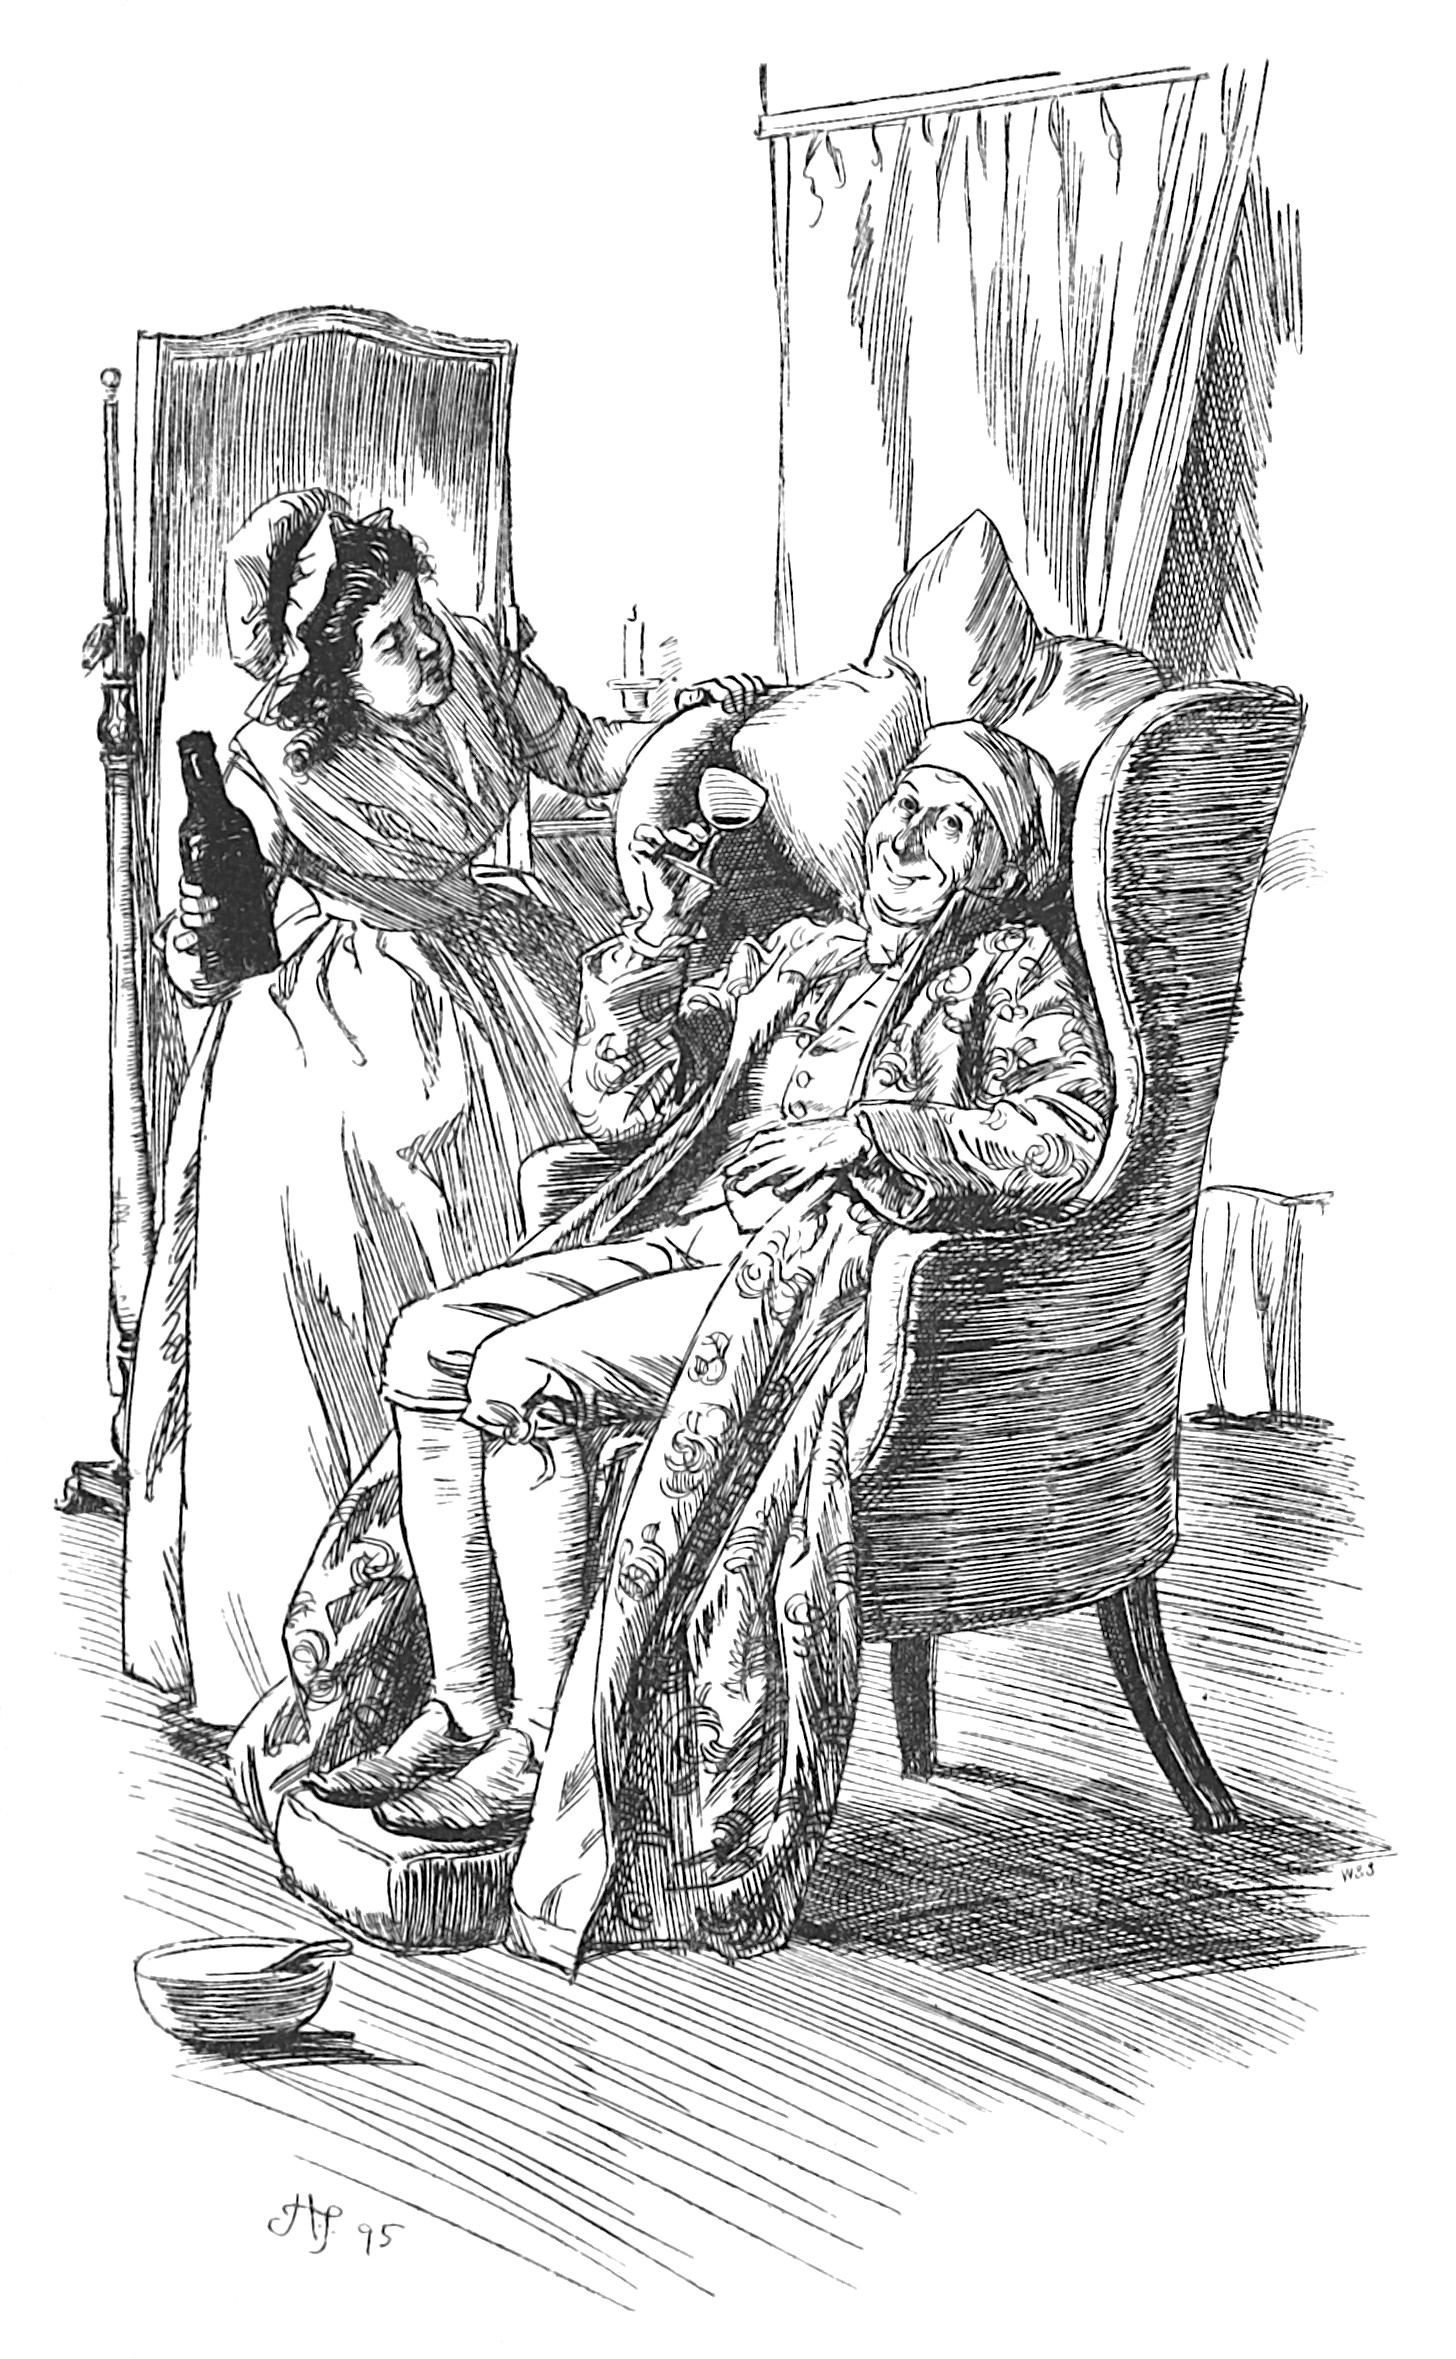
\includegraphics[width=.8\linewidth]{30fond}
		\caption{How fond he was of it!}
	\end{figure}
\end{a4}

\begin{letter}
	\begin{figure}[tbph]
		\centering
		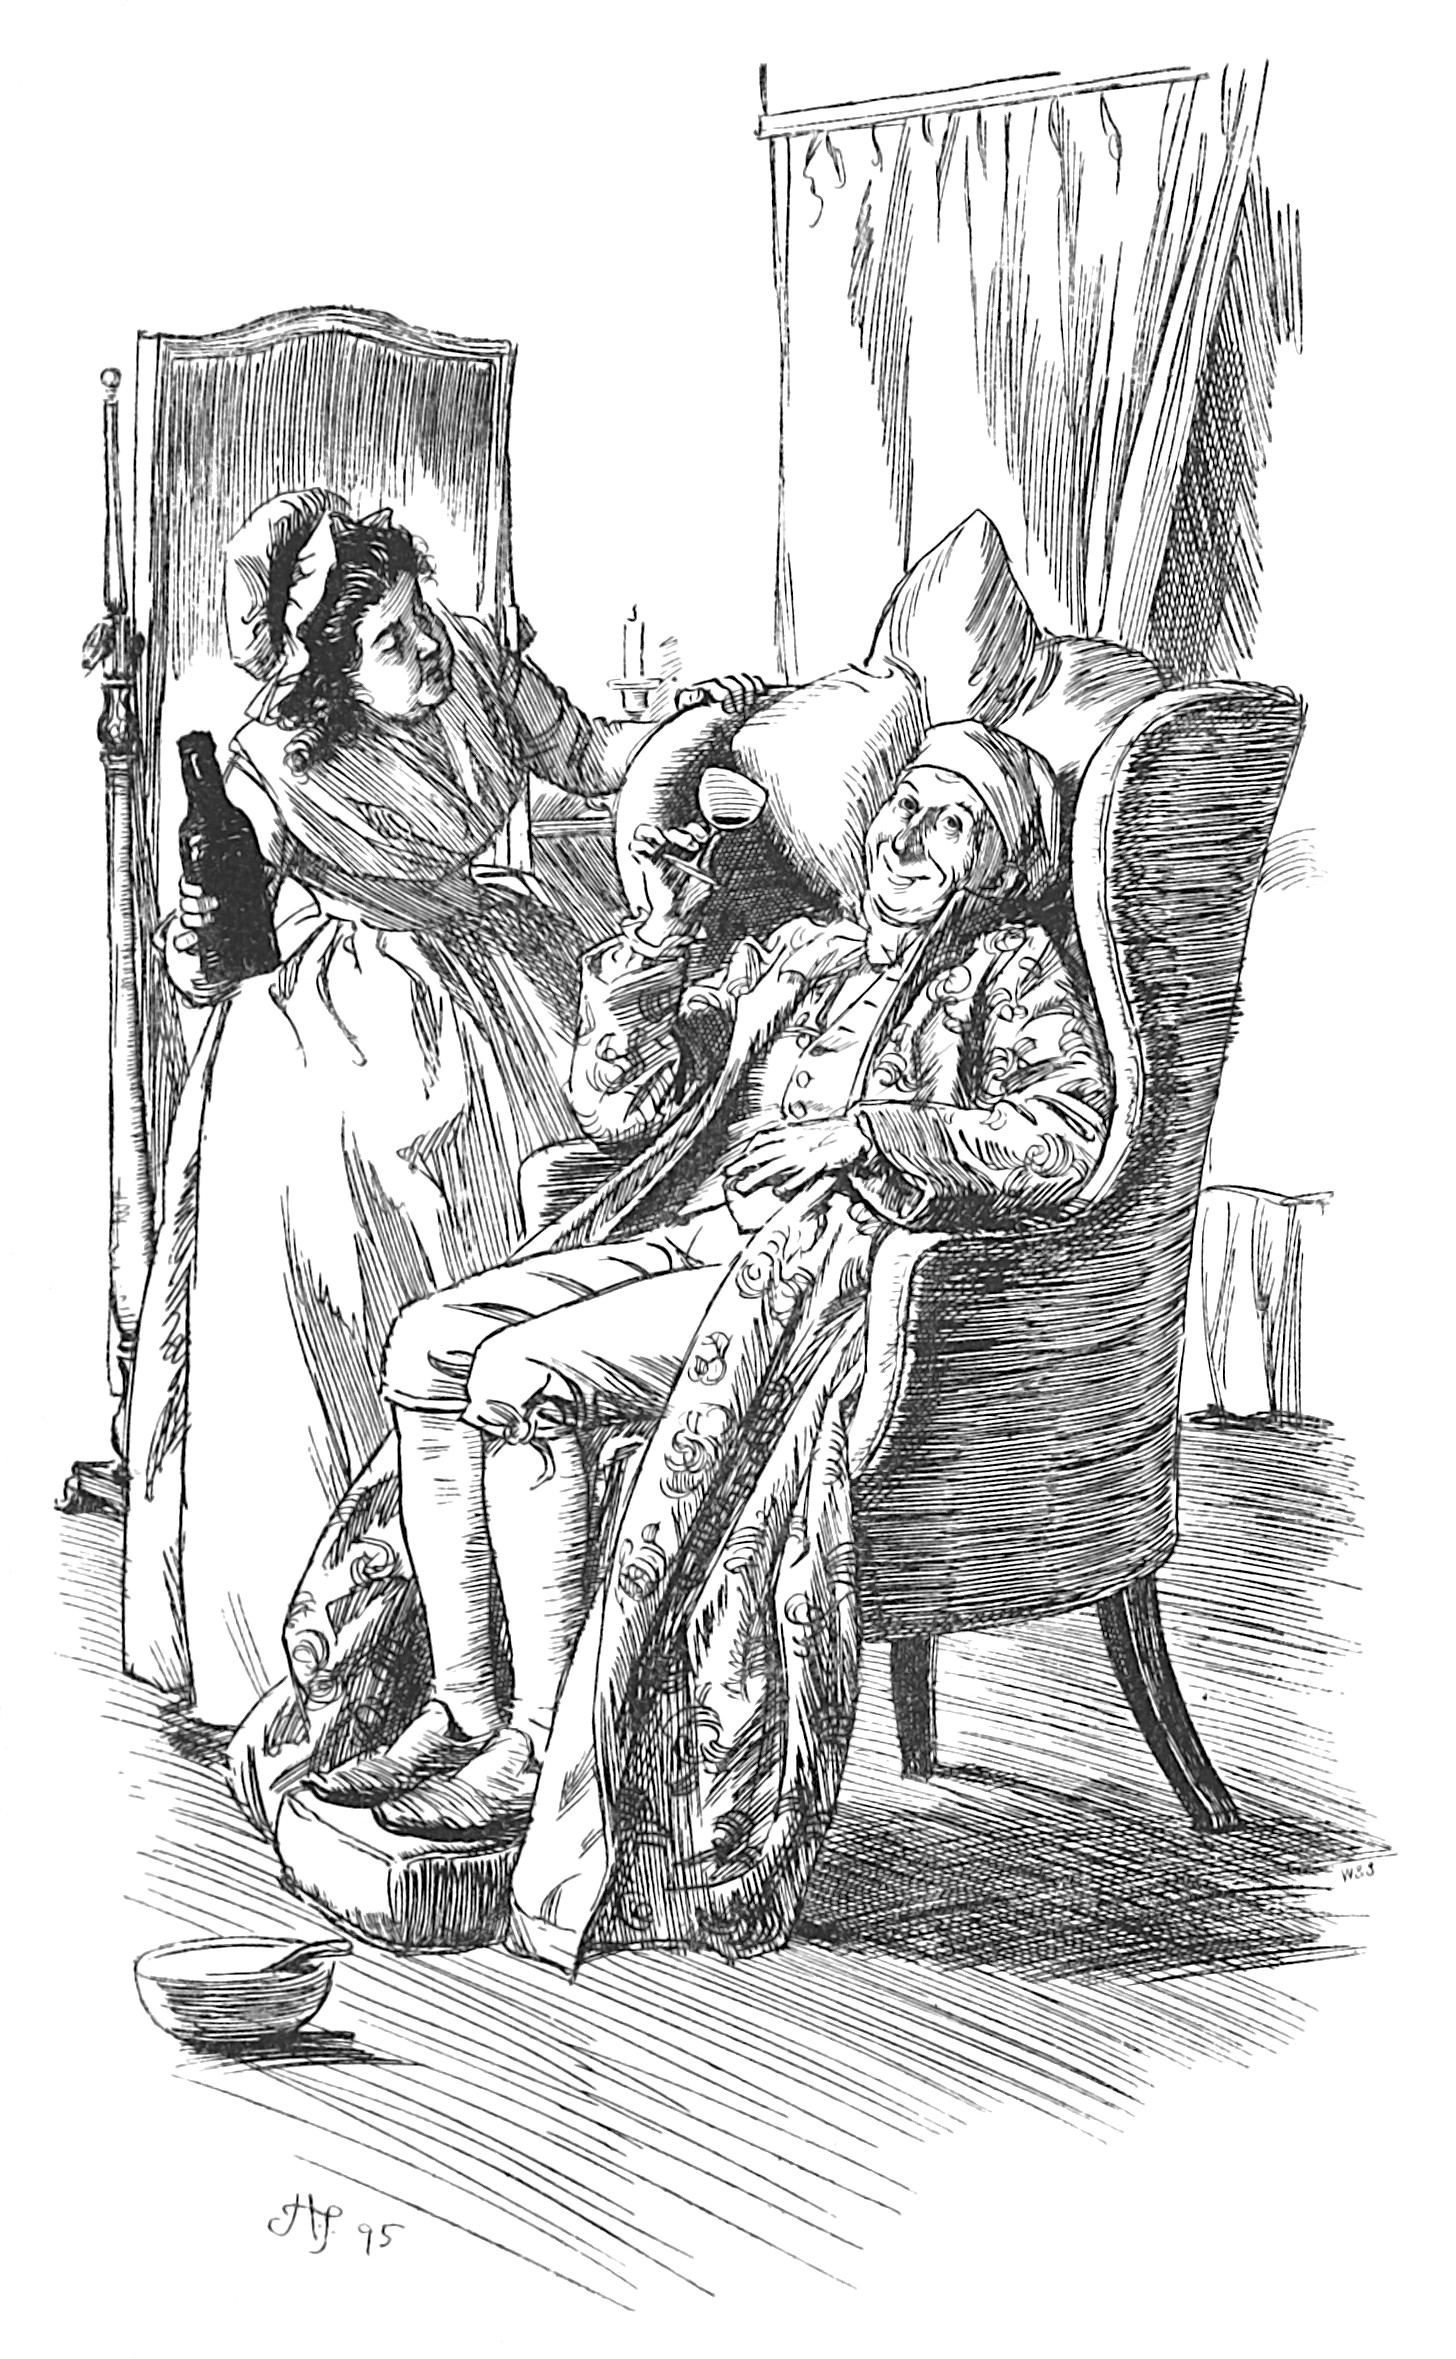
\includegraphics[width=\linewidth]{30fond}
		\caption{How fond he was of it!}
	\end{figure}
\end{letter}



<Dear Ma'am,> replied Elinor, smiling at the difference of the complaints for which it was recommended, <how good you are! But I have just left Marianne in bed, and, I hope, almost asleep; and as I think nothing will be of so much service to her as rest, if you will give me leave, I will drink the wine myself.>

Mrs Jennings, though regretting that she had not been five minutes earlier, was satisfied with the compromise; and Elinor, as she swallowed the chief of it, reflected, that though its effects on a colicky gout were, at present, of little importance to her, its healing powers, on a disappointed heart might be as reasonably tried on herself as on her sister.

Colonel Brandon came in while the party were at tea, and by his manner of looking round the room for Marianne, Elinor immediately fancied that he neither expected nor wished to see her there, and, in short, that he was already aware of what occasioned her absence. Mrs Jennings was not struck by the same thought; for soon after his entrance, she walked across the room to the tea-table where Elinor presided, and whispered, <The Colonel looks as grave as ever you see. He knows nothing of it; do tell him, my dear.>

He shortly afterwards drew a chair close to hers, and, with a look which perfectly assured her of his good information, inquired after her sister.

<Marianne is not well,> said she. <She has been indisposed all day, and we have persuaded her to go to bed.>

<Perhaps, then,> he hesitatingly replied, <what I heard this morning may be—there may be more truth in it than I could believe possible at first.>

<What did you hear?>

<That a gentleman, whom I had reason to think—in short, that a man, whom I \textit{knew} to be engaged—but how shall I tell you? If you know it already, as surely you must, I may be spared.>

<You mean,> answered Elinor, with forced calmness, <Mr Willoughby's marriage with Miss Grey. Yes, we \textit{do} know it all. This seems to have been a day of general elucidation, for this very morning first unfolded it to us. Mr Willoughby is unfathomable! Where did you hear it?>

<In a stationer's shop in Pall Mall, where I had business. Two ladies were waiting for their carriage, and one of them was giving the other an account of the intended match, in a voice so little attempting concealment, that it was impossible for me not to hear all. The name of Willoughby, John Willoughby, frequently repeated, first caught my attention; and what followed was a positive assertion that every thing was now finally settled respecting his marriage with Miss Grey—it was no longer to be a secret—it would take place even within a few weeks, with many particulars of preparations and other matters. One thing, especially, I remember, because it served to identify the man still more:—as soon as the ceremony was over, they were to go to Combe Magna, his seat in Somersetshire. My astonishment!—but it would be impossible to describe what I felt. The communicative lady I learnt, on inquiry, for I stayed in the shop till they were gone, was a Mrs Ellison, and that, as I have been since informed, is the name of Miss Grey's guardian.>

<It is. But have you likewise heard that Miss Grey has fifty thousand pounds? In that, if in any thing, we may find an explanation.>

<It may be so; but Willoughby is capable—at least I think>—he stopped a moment; then added in a voice which seemed to distrust itself, <And your sister—how did she\longdash>

<Her sufferings have been very severe. I have only to hope that they may be proportionately short. It has been, it is a most cruel affliction. Till yesterday, I believe, she never doubted his regard; and even now, perhaps—but \textit{I} am almost convinced that he never was really attached to her. He has been very deceitful! and, in some points, there seems a hardness of heart about him.>

<Ah!> said Colonel Brandon, <there is, indeed! But your sister does not—I think you said so—she does not consider quite as you do?>

<You know her disposition, and may believe how eagerly she would still justify him if she could.>

He made no answer; and soon afterwards, by the removal of the tea-things, and the arrangement of the card parties, the subject was necessarily dropped. Mrs Jennings, who had watched them with pleasure while they were talking, and who expected to see the effect of Miss Dashwood's communication, in such an instantaneous gaiety on Colonel Brandon's side, as might have become a man in the bloom of youth, of hope and happiness, saw him, with amazement, remain the whole evening more serious and thoughtful than usual.